\documentclass[]{book}
\usepackage{lmodern}
\usepackage{amssymb,amsmath}
\usepackage{ifxetex,ifluatex}
\usepackage{fixltx2e} % provides \textsubscript
\ifnum 0\ifxetex 1\fi\ifluatex 1\fi=0 % if pdftex
  \usepackage[T1]{fontenc}
  \usepackage[utf8]{inputenc}
\else % if luatex or xelatex
  \ifxetex
    \usepackage{mathspec}
  \else
    \usepackage{fontspec}
  \fi
  \defaultfontfeatures{Ligatures=TeX,Scale=MatchLowercase}
\fi
% use upquote if available, for straight quotes in verbatim environments
\IfFileExists{upquote.sty}{\usepackage{upquote}}{}
% use microtype if available
\IfFileExists{microtype.sty}{%
\usepackage{microtype}
\UseMicrotypeSet[protrusion]{basicmath} % disable protrusion for tt fonts
}{}
\usepackage[margin=1in]{geometry}
\usepackage{hyperref}
\hypersetup{unicode=true,
            pdftitle={Sentinel Asia Handbook},
            pdfauthor={Firman Hadi and Syams Nashrrullah},
            pdfborder={0 0 0},
            breaklinks=true}
\urlstyle{same}  % don't use monospace font for urls
\usepackage{natbib}
\bibliographystyle{apalike}
\usepackage{longtable,booktabs}
\usepackage{graphicx,grffile}
\makeatletter
\def\maxwidth{\ifdim\Gin@nat@width>\linewidth\linewidth\else\Gin@nat@width\fi}
\def\maxheight{\ifdim\Gin@nat@height>\textheight\textheight\else\Gin@nat@height\fi}
\makeatother
% Scale images if necessary, so that they will not overflow the page
% margins by default, and it is still possible to overwrite the defaults
% using explicit options in \includegraphics[width, height, ...]{}
\setkeys{Gin}{width=\maxwidth,height=\maxheight,keepaspectratio}
\IfFileExists{parskip.sty}{%
\usepackage{parskip}
}{% else
\setlength{\parindent}{0pt}
\setlength{\parskip}{6pt plus 2pt minus 1pt}
}
\setlength{\emergencystretch}{3em}  % prevent overfull lines
\providecommand{\tightlist}{%
  \setlength{\itemsep}{0pt}\setlength{\parskip}{0pt}}
\setcounter{secnumdepth}{5}
% Redefines (sub)paragraphs to behave more like sections
\ifx\paragraph\undefined\else
\let\oldparagraph\paragraph
\renewcommand{\paragraph}[1]{\oldparagraph{#1}\mbox{}}
\fi
\ifx\subparagraph\undefined\else
\let\oldsubparagraph\subparagraph
\renewcommand{\subparagraph}[1]{\oldsubparagraph{#1}\mbox{}}
\fi

%%% Use protect on footnotes to avoid problems with footnotes in titles
\let\rmarkdownfootnote\footnote%
\def\footnote{\protect\rmarkdownfootnote}

%%% Change title format to be more compact
\usepackage{titling}

% Create subtitle command for use in maketitle
\newcommand{\subtitle}[1]{
  \posttitle{
    \begin{center}\large#1\end{center}
    }
}

\setlength{\droptitle}{-2em}
  \title{Sentinel Asia Handbook}
  \pretitle{\vspace{\droptitle}\centering\huge}
  \posttitle{\par}
  \author{Firman Hadi and Syams Nashrrullah}
  \preauthor{\centering\large\emph}
  \postauthor{\par}
  \predate{\centering\large\emph}
  \postdate{\par}
  \date{2018-06-28}

\usepackage{booktabs}

\begin{document}
\maketitle

{
\setcounter{tocdepth}{1}
\tableofcontents
}
\chapter*{Preface}\label{preface}
\addcontentsline{toc}{chapter}{Preface}

Due to the nature of the Sentinel Asia (SA) works which are related to
disaster response, Value Added Products (VAPs) are expected to be
produced as soon as the data are available. The book serves as a
guidance for streamlining the process and techniques for data processing
related to SA Activities. Hence, it is expected that the book will help
in reaching the objective.

\chapter{Preparation}\label{preparation}

To conduct Sentinel Asia activities, there are several things that need
to be prepared, (1) Hardware, (2) softwares and (3) Standard Operational
Procedures.

\section{Hardwares}\label{hardwares}

There are three main computers used for Sentinel Asia works, (1) CentOS
Linux , (2) Windows PC and (3) MacPro. CentOS Linux is used as Image
Management System, activating scripts for PDAN website and serve as data
storage downloaded from Sentinel Asia website. Windows PC is used to
handle processing data related to flood, while MacPro is used to process
data related to geological hazard such as volcano and earthquake.

\section{Softwares}\label{softwares}

\section{Standard Operational
Procedures}\label{standard-operational-procedures}

\chapter{Introduction}\label{intro}

Sentinel Asia is a voluntary initiative to provide satellite data at a
time of a disaster, and to coordinate support in collaboration with data
provider nodes (DPNs), data analysis nodes (DANs), and disaster
management organizations (DMOs) in the Asia-Pacific region. Data
analyses and value added product (VAP) generation is done through
several agencies including the GIC/AIT, which is the Primary Data
Analysis Node (P-DAN). Moreover, Sentinel Asia also supports activities
on disaster risk reduction (DRR) to its member countries in the region.
In this respect, technical and disaster management organizations are
members of Sentinel Asia and are known as joint project team members
(JPTM).

The time lapse of work-flow from a disaster occurrence to the product
delivery stage is an important factor that has a high impact on DRR
activities. The work-flow is a process chain consisting of various
stages such as an emergency observation request (EOR), Sentinel Asia
activation, satellite observations, image processing and analyses,
value-added product (VAPs) generation, product delivery and sharing. It
is important to reduce the time gaps in this process chain. The GIC/AIT
has provided the service as the P-DAN during the contract period.

The main components of the works are (1) the Project Manager (PM)
activities of the International Disaster Charter (IDC) and (2)
generation, provision and evaluation of Value Added Products (VAPs).

All the service for Sentinel Asia activation is provided by effectively
communicating with the Sentinel Asia Secretariat and collecting related
information in order to identify the severity and to monitor the
progress after an activation. Assistance is provided to the authorized
users (AU) of the Asian Disaster Reduction Center (ADRC) member
countries to receive data and products in a timely manner and to share
VAPs with the ADRC and its member countries. After the VAPs are
generated, close communication is maintained during the contract period
with DAN members of the Sentinel Asia-activated countries.

\section{Project Manager (PM) Activities of International Disaster
Charter
(IDC)}\label{project-manager-pm-activities-of-international-disaster-charter-idc}

When a major disaster occurs, the Asian Disaster Reduction Center (ADRC)
can escalate a Sentinel Asia emergency observation request to the
International Disaster Charter (IDC). A project manager (PM), such as
the GIC/AIT, will be nominated from relevant national agencies or
international organizations. The PM role is to ensure effective
communication between the data providers or partner agencies (PA), value
added companies/resellers and authorized users (AU). The PM will
coordinate the activation, ensuring that the acquisition of satellite
images is under way, managing the generation of products or information,
and making sure that the products are delivered to the users according
to their needs and expectations. The Charter activation is considered
closed 30 days after the initial activation date or when the end users
have enough products for their requirements. The PM will then have to
submit a report to the Charter Executive Secretariat (the member of the
PA that nominated the PM -- in this case the JAXA) - within 45 days of
the initial activation date through email or the COS-2 system. The PM
report will conclude the PM's work for this Charter activation.

\section{Sentinel Asia Activities}\label{sentinel-asia-activities}

As the primary data analysis node (P-DAN) of Sentinel Asia, the GIC/AIT
has been effectively communicating with the Sentinel Asia
Secretariat/ADRC and coordinating the response of DAN members for each
emergency observation request. The GIC/AIT analyzed satellite data which
provided by the data provider nodes (DPNs), and then created VAPs and
shared such satellite-based disaster information products to end users
in timely manner.

\chapter{Sentinel Asia Activation Response
Workflow}\label{sentinel-asia-activation-response-workflow}

Here is a the general procedure that should be followed during the
Sentinel Asia Activation.

\section{Immediate Response}\label{immediate-response}

\subsection{Work management}\label{work-management}

\begin{enumerate}
\def\labelenumi{\arabic{enumi}.}
\tightlist
\item
  Create an activation folder in Kepler
\item
  Track the observation plan of satellite data
\end{enumerate}

\subsection{Initial communication with requestor/end
user}\label{initial-communication-with-requestorend-user}

\begin{enumerate}
\def\labelenumi{\arabic{enumi}.}
\tightlist
\item
  Confirm the affected areas
\item
  Update the most recent ground situation
\item
  Identify the user needs of VAPs
\item
  Request the user to share ground information
\end{enumerate}

\subsection{Download/preparing vector
data}\label{downloadpreparing-vector-data}

The data for many of Asian countries have been prepared in ArcGIS
Geodatabase. Please see Appendices to see how to connect to the
Geodatabase.

\subsection{Download other relevant
data}\label{download-other-relevant-data}

\begin{enumerate}
\def\labelenumi{\arabic{enumi}.}
\tightlist
\item
  Download SRTM
\item
  Download WorldPop
\end{enumerate}

\subsection{Initial data processing}\label{initial-data-processing}

\begin{enumerate}
\def\labelenumi{\arabic{enumi}.}
\tightlist
\item
  Create project in ArcGIS Pro
\item
  Connect to the Country DataBase
\item
  Identify the affected admin area
\item
  Calculate slope from DEM
\end{enumerate}

\subsection{ArcGIS Online}\label{arcgis-online}

\begin{enumerate}
\def\labelenumi{\arabic{enumi}.}
\tightlist
\item
  Create a project for the activation
\item
  Create a rainfall monitoring tab
\item
  Create a tab for social media integration
\end{enumerate}

\subsection{PDAN System}\label{pdan-system}

\begin{enumerate}
\def\labelenumi{\arabic{enumi}.}
\tightlist
\item
  Activate email notification
\item
  Update PDAN website (front page)
\item
  Create PDAN forum
\item
  Integrate ArcGIS Online
\end{enumerate}

\subsection{Prepare activation report (using
template)}\label{prepare-activation-report-using-template}

\begin{enumerate}
\def\labelenumi{\arabic{enumi}.}
\tightlist
\item
  Write `Overview'
\item
  Write `Description of Disaster Situation'
\item
  Write `Disaster Affected Areas'
\item
  Write `Data Availability'
\item
  Write `Communication'
\end{enumerate}

\section{Data provision and VAP
generation}\label{data-provision-and-vap-generation}

\subsection{Work management}\label{work-management-1}

\begin{enumerate}
\def\labelenumi{\arabic{enumi}.}
\tightlist
\item
  Call for a meeting, if necessary
\item
  Assign staffs available for data processing
\end{enumerate}

\subsection{Communication with
requestor/end-user}\label{communication-with-requestorend-user}

\subsubsection{Check and re-check}\label{check-and-re-check}

Check the draft of VAP by overlaying it with OpenStreetMap data or other
GIS services (Google etc.)

\chapter{Standard Operational Procedure
(SOP)}\label{standard-operational-procedure-sop}

This chapter is arranged to different sections according to the most
frequent type of disaster in previous Sentinel Asia Activities. On each
section, the explanation will be based on available data.

\section{Data processing}\label{data-processing}

\subsection{Flood}\label{flood}

\subsubsection{SAR}\label{sar}

\paragraph{ALOS-2}\label{alos-2}

Before processing the data, it is better to check the processing level
from the filename.

\paragraph{Level 1.5}\label{level-1.5}

\paragraph{Level 2.1}\label{level-2.1}

\subsubsection{Optical data}\label{optical-data}

\subsubsection{Google Earth Engine (GEE)}\label{google-earth-engine-gee}

\subsection{Earthquake}\label{earthquake}

\subsection{Volcano}\label{volcano}

\subsection{Landslide}\label{landslide}

\subsection{Glacier Lake Outburst
Flood}\label{glacier-lake-outburst-flood}

\subsection{Forest Fire}\label{forest-fire}

\section{Data Layout}\label{data-layout}

\subsection{Check and re-check}\label{check-and-re-check-1}

\begin{enumerate}
\def\labelenumi{\arabic{enumi}.}
\tightlist
\item
  Check and re-check the draft of VAP before uploading to SA server.
\item
  Compare the geometry with other available online data \#\# Data Upload
  to Server
\end{enumerate}

\chapter{PC/Servers Management}\label{pcservers-management}

\section{ArcGIS Server}\label{arcgis-server}

\section{SQL Server}\label{sql-server}

\subsection{Maintenance}\label{maintenance}

\subsubsection{Database Backup}\label{database-backup}

\subsubsection{Database Compression}\label{database-compression}

\url{http://desktop.arcgis.com/en/arcmap/10.5/manage-data/geodatabases/compress-versioned-geodatabase.htm}

\section{PDAN Website}\label{pdan-website}

\section{Image Management System}\label{image-management-system}

\subsection{Connection}\label{connection}

\section{Sentinel-PC}\label{sentinel-pc}

\subsection{Connection}\label{connection-1}

\subsection{Softwares}\label{softwares-1}

\section{MacPro}\label{macpro}

\subsection{Connection}\label{connection-2}

\begin{itemize}
\tightlist
\item
  From Mac
\end{itemize}

-- Click Spotlight and type vnc://203.159.21.212

\begin{figure}

{\centering 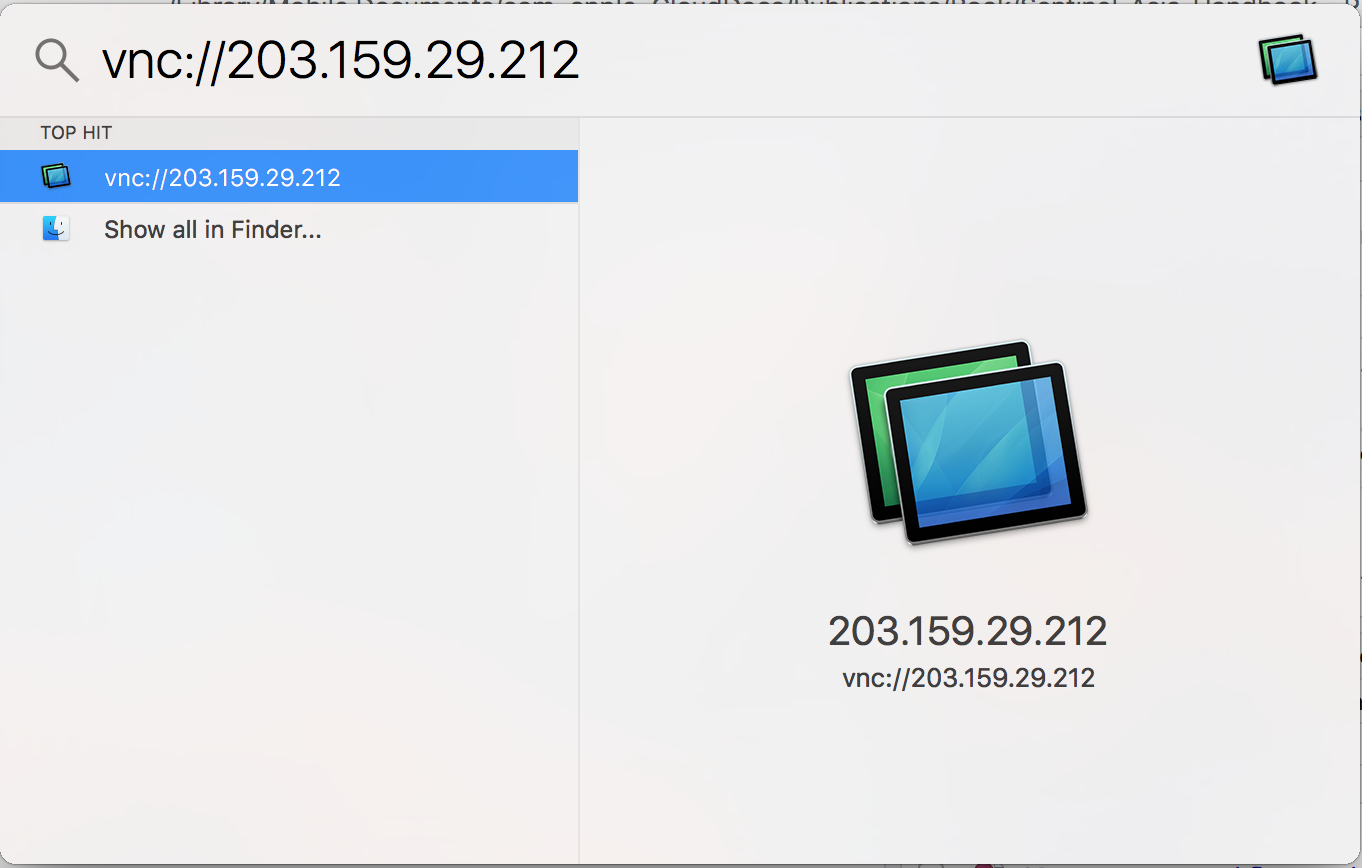
\includegraphics[width=0.7\linewidth]{img/fig41_vnc} 

}

\caption{Accessing MacPro using VNC}\label{fig:fig41a}
\end{figure}

-- Type username and password

\begin{figure}

{\centering 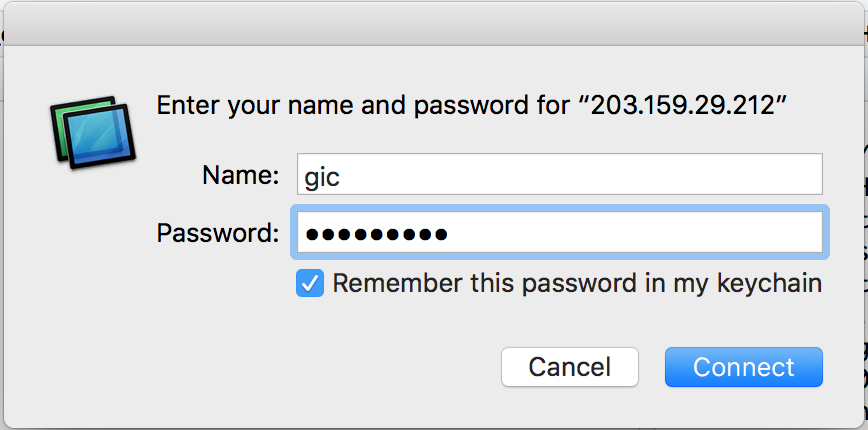
\includegraphics[width=0.7\linewidth]{img/fig41_vnc1} 

}

\caption{Type username and password}\label{fig:fig41b}
\end{figure}

-- Mac environment after login

\begin{figure}

{\centering \includegraphics[width=0.7\linewidth]{img/fig41_vnc2} 

}

\caption{Mac environment}\label{fig:fig41c}
\end{figure}

\begin{itemize}
\tightlist
\item
  From Windows
\end{itemize}

\subsection{Softwares}\label{softwares-2}

\chapter*{Appendices}\label{appendices}
\addcontentsline{toc}{chapter}{Appendices}

\subsection*{ArcGIS Enterprise Geodatabase
connection}\label{arcgis-enterprise-geodatabase-connection}
\addcontentsline{toc}{subsection}{ArcGIS Enterprise Geodatabase
connection}

\subsection*{Useful Links}\label{useful-links}
\addcontentsline{toc}{subsection}{Useful Links}

\subsection*{ArcGIS Pro scripts}\label{arcgis-pro-scripts}
\addcontentsline{toc}{subsection}{ArcGIS Pro scripts}

\subsection*{Generalization script}\label{generalization-script}
\addcontentsline{toc}{subsection}{Generalization script}

\bibliography{book.bib,packages.bib}


\end{document}
